\documentclass[../thesis.tex]{subfiles}
\graphicspath{{\subfix{../assets/}}}
\begin{document}


\chapter{Inverse Language Modeling}
\label{chap:inversion}

Large Language Models (LLMs) nowadays excel in natural language tasks, allowing us to perform multiple NLP tasks with a single foundation model, often beating previous state-of-the-art solutions. Thanks to recent studies in reasoning \citep{xu2025largereasoningmodelssurvey}, LLMs can solve even more complex tasks, which was not possible before when they had to give an answer immediately after the user prompt.
Yet LLMs are prone to hallucinations. Moreover, they are sensitive to adversarial inputs, as observed in the introduction. These phenomena highlight a possible risk for backdoors and bad behaviour induced by a bad actor using a model.
Because of all of that, it is obvious the need for Adversarial Training (AT) also for LLMs, similarly to what happened in the past to image deep classifiers, leaving adversarial text perturbations an open challenge.

In this context, \emph{robust} means being less sensitive to input prompts, and \emph{grounded} means ``making LLMs know what they have been asked about'', not simply predicting the most likely next token in the sentence.
Indeed, LLMs do not know what they are talking about \citep{guo2024language}, supporting the idea of LLMs as complex stochastic parrots.

In this chapter, we introduce \textbf{Inverse Language Modeling} (ILM), which takes inspiration from years of progress on adversarial robustness in deep classifiers.
LLMs are trained in forward-mode, predicting the next token in a self-supervised way.
ILM, instead, focuses on the idea that should be possible to have a meaning of the spoken sentence even backwards: given $\by$ (the answer or the LLM proposed continuation), is the LLM aware of the text prompt $\bx$ it was conditioned on?
This does not mean to train the LLM with a reversed corpus, but instead predicting based on the value of the gradients on the input, as in \cref{fig:inverse_lm_idea_schema}. This should be possible because of the fact illustrated in \cref{fig:llm_gradients_changing_embedding}, where we observed that the gradients can have the notion of the overall sentence.

This method could potentially allow for a security red team to better investigate and study malicious prompts $\bx$ that could lead to the generation of an undesired output $\by$, by simply inverting the LM, after being correctly fine-tuned as in the procedure illustrated in this chapter.

We will use ILM at training time, while at test time we exploit the GCG algorithm to find, given an original text prompt $\bx$ and the completion $\by$, a new nonsensical $\bxa$ such that the loss $\Loss(\bxa,\by;\net) \ll \Loss(\bx,\by;\net)$, where $\Loss$ is the next-token prediction loss of the LLM and $\net$ are LLM’s parameters. We prove there exists a nonsensical prompt $\bxa$ that ``connects'' better to $\by$ (lower loss) than the natural $\bx$.

\begin{figure}
\centering
\vspace{0.5cm}
\begin{overpic}[width=0.7\linewidth]{inverse-lm/forward_backward_llm}
    \put(5.5,0){$\bx_1$}\put(19.5,0){$\bx_2$}\put(33.5,0){$\bx_3$}
    \put(5.5,27){$\bx_2$}\put(19.5,34){$\bx_3$}\put(33.5,44){$\bx_4$}
    \put(60,43.5){$\bx_2$}\put(72,43.5){$\bx_3$}\put(87,43.5){$\bx_4$}
    \put(60,0){$\bx_1$}\put(72,10){$\bx_2$}\put(87,18){$\bx_3$}
    \put(17,59.5){{\footnotesize \textbf{Now}}}
    \put(68,59.5){{\footnotesize \textbf{Proposed}}}
    \put(0,55){{\footnotesize Autoregressive forward}}
    \put(55,55){{\footnotesize Autoregressive backward}}
    \put(5,49){{\scriptsize $p(\bx_i|\bx_1,\ldots,\bx_{i-1})$}}
    \put(50,49){{\scriptsize$p\big(\bx_{i-1}| \nabla_{\bx_{i-1}}p(\bx_i|\bx_1,\ldots,\bx_{i-1})\big)$}}
\end{overpic}
\caption{Inverse Language Modeling}
\label{fig:inverse_lm_idea_schema}
\end{figure}


\section{Inverting the first token}
As a preliminary experiment to have some experimental data to discuss to support our ideas, but also not to consume too much computational power for the first experiment, we decided to train our LLM to predict the first token of a sentence.

To keep the entropy in the token classification somehow limited, we adopted the \textbf{TinyStories dataset} \citep{eldan2023tinystoriessmalllanguagemodels}
\footnote{\url{https://huggingface.co/datasets/fhswf/TinyStoriesV2_cleaned}},
which allows us to work with synthetically generated (GPT-4) short stories that only use a small vocabulary.

In order to perform flexible experiments, even the tokenizer is trained by ourselves, allowing us to set a specific vocabulary size to reach applying the Byte-Pair Encoding (BPE) algorithm \citep{gage1994new-bytepairencoding-bpe}.
Then, the model is trained from scratch, reaching good results in just a bunch of epochs, due to the simplicity of the corpus we used, proceeding by using, at first, the same hyperparameters of the original experiment
\footnote{\url{https://huggingface.co/raincandy-u/TinyStories-656K\#full-training-arguments}}.

To implement the inversion goal, we use the gradients with respect to the embeddings of the input sequence, in the same way as if it was the last hidden state.
This has a twofold effect:
\begin{enumerate}
    \item The last hidden state has necessary knowledge of the overall sentence to predict the next token, so the gradients of the embeddings
    \item Because of \textbf{weight tying} \citep{press2017usingoutputembeddingimprove-weighttying}, the weights of the classification head and the embeddings layer are exactly the same at any step of the training process - this induced parallelism is exploited here even further
\end{enumerate}

Because of the weight tying parallelism and recalling \cref{fig:llm_gradients_changing_embedding}, we can threat $\nabla_{e_i}$ to predict the token $x_i$.
More formally, the backward prediction $\mathbf{\hat{y}}$ is obtained as in \cref{eq:inverse_lm_backward_prediction_base}.
To perform this task, we need to add a new regularization term to the standard CE loss function. The final loss is expressed in \cref{eq:inverse_lm_backward_loss_base}.

\begin{equation}
\begin{split}
    \loss_{CE} &= CE(\by_\text{true}, \by_\text{pred}) \\
    \bg_i &= \text{LayerNorm}(\nabla_{e_i}\loss_{CE}) \\
    \bz_i &= \bw_\text{LM\_head} \; \bg_i \\
    \mathbf{\hat{y}}_i &= \text{softmax}(\bz_i)
\end{split}
\label{eq:inverse_lm_backward_prediction_base}
\end{equation}

\begin{equation}
\loss = 
\underbrace{CE(\by_\text{true}, \by_\text{pred})}_\text{Forward: from the input x, encode y}
+
\underbrace{\lambda\ CE(\bx, \mathbf{\hat{y}})}_\text{Backward: from y, decode back x}
\label{eq:inverse_lm_backward_loss_base}
\end{equation}

This approach has the potential downside of being different between training and test time.
Looking more in deep at the formulas, it is visible that the backward prediction target $\bx$ is already given, while at test time we have to replace it with a random token, being a valid vocabulary token or the \texttt{[PAD]} padding special token.
However, this is efficient for training since we do not need multiple forward passes to the model, requiring us to save in memory only one instance of the activations because of the single forward pass.

\subsection{Considerations on the classification strategy}
A question that may arise is why we decided to multiply the gradients by the LM head weights matrix and applying softmax.
A naive approach could be to directly use $\bg_i$ as the embedding of the target token and classify the correct token simply by looking at the token with the nearest embedding, using $L_2$ distance or cosine similarity.
This has several major downsides:
\begin{enumerate}
    \item It would lead to the same problem observed with the toy example in \cref{sec:pag__pag_variants_strategies} with the so called ``PAG identity'' approach, where the gradients ideally reconstruct the input
    \item It would not have exploited the unique symmetry introduced by weight tying, for which the weights matrix of the embeddings layer and the LM head are exactly the same
    \item It would not have lead to a probability distribution over the tokens in the vocabulary
\end{enumerate}

Instead, treating $\bg_i$ exactly the same as if it was the last hidden state that predicts token $\bx_i$, allows us to map this gradient to an image of something that is linked to the expected outcome, instead of directly the input.
Moreover, we can apply the same techniques that are commonly used in forward test mode, like Beam Search, Top-K Sampling and so on and so forth.
The parallelism is highlighted in the illustration in \cref{fig:grad_lm_head_parallelism}.

Using a simple measure of distance would make the loss \textbf{non-contrastive}.
This means that there is a much higher risk of \textbf{collapse} of the hidden states obtained from the gradients during the backward operational mode.
It is clearly justified by the meaning of the loss itself: it imposes the embeddings of a target token $\be_i$ to be as similar as possible to the gradients $\nabla_{\be_j} \loss$. However, nothing is said about the dissimilarity between embeddings that should not relate each other. The optimal solution in this setting would be to assign the same value to every embedding.
Since this would just be a single regularization term in the loss (also the CE loss of the language model participates in the overall loss), we only talk about a high risk of going in the direction of a collapse, not a certainty.

On the other hand, having a tensor that can be interpreted as the output logits, we can introduce the \textbf{softmax} as a standard part of the cross-entropy loss, introducing the contrastive part previously missing. This allows to keep clear separation hyperplanes between the different hidden states that lead to a specific token prediction.

\begin{figure}
    \centering
    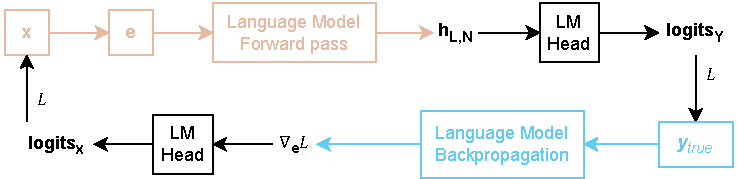
\includegraphics[width=\linewidth]{assets/inverse-lm/grad_lm_head_parallelism.drawio.pdf}
    \caption{Parallelism between the last hidden state and the gradients on the embeddings}
    \label{fig:grad_lm_head_parallelism}
\end{figure}

Aside from that, it must be highlighted that all these methods do not work if we omit the \textbf{LayerNorm} function application.
We questioned why this was the case, so we started to delve deeper into the sequence of applied functions, in a standard forward pass, before the matrix multiplication with the final LM Head.
Based on the internal code analysis, it was observed that the final hidden state includes a value previously passed to the \texttt{T5LayerNorm}%
\footnote{\url{https://github.com/huggingface/transformers/blob/fa3c3f9cab1c45b449bd57e238c511c79637e314/src/transformers/models/t5/modeling\_t5.py\#L241}}
layer, which rescales the variance of the input tensor, without subtraction of mean and the bias parameter.

\begin{equation}
\begin{split}
    \sigma &= \sqrt{\frac{1}{D} \sum_{i=0}^D \bx_i^2 + \varepsilon} \\
    \bx' &= \alpha \frac{\bx}{\sigma}
\end{split}
\end{equation}


\subsection{Variants}
As immediately visible, this is not a simple problem. Because of that, multiple approaches have been implemented and compared, here discussed.
The common denominator between all of them is the approach highlighted in the previous section: the gradient on the tokens embedding $\nabla_{e_i}$ is forwarded to the LM Head $\bw$ classifier. The difference lies in how this gradient is obtained and used in the final $\loss$ loss function.
To briefly give them a name:
\begin{itemize}
    \item \textbf{identity}: compute $\nabla_{e_i}$ on a simple forward pass with the usual Cross-Entropy Loss, then impose the logits obtained from $\bw^T \cdot \nabla_{e_i}$ to match the token $\bx_i$
    \item \textbf{inv-first}: after replacing the first input token $\bx_0$ with \texttt{<|pad|>}, leaving the labels unchanged, do a forward pass and compute $\nabla_{e_i}$ (now, this gradient cannot carry information about the token $\bx_0$ to predict)
    \item \textbf{bert-like}: replace 10\% of tokens, randomly selected, both as input tokens and target label tokens, then the same prediction procedure is followed; this method is heavily inspired by BERT \citep{devlin2019bert}, in which the model should understand the meaning of the sentence - here, the LLM is supposed to be an autoregressive LM in the forward pass, while being a model like BERT when computing the backward pass.
\end{itemize}


\subsection{Inverse LM Evaluation}
\label{sec:ilm_first_evaluation}
The evaluation procedure consists of multiple steps:
\begin{enumerate}
    \item Validation loss identifies the value of the loss in the same setting as the training loop
    \item Validation accuracy indicates the prediction capabilities of the model in the same setting as the training, serving as baseline indicators of model fit and predictive performance
    \item Inverse LM accuracy measures the ability of a model to reconstruct a masked token $\bx_i$ from its gradients, given the remaining context; this provides a direct assessment of the backward prediction mechanism.
\end{enumerate}

To compute the Inverse LM accuracy, a token $\bx_i$ must be predicted, at position $i$.
The input of the model is the original sentence, where the $i$-th token is replaced with a placeholder, concatenated by all the following tokens.
Formally:
\begin{itemize}
    \item we aim to predict the $i$-th token, where $1 \leq i < N$
    \item given an input sentence $\bx = \bx_1, \bx_2, ..., \bx_{N-1}$
    \item the target labels $\by = \bx_2, \bx_3, ..., \bx_N$
    \item the input is $\bx' = \texttt{<|pad|>}, \bx_{i+1}, ..., \bx_{N-1}$
    \item the CE loss is computed with the target labels defined as $\by' = \bx_{i+1}, ..., \bx_{N-1}, \bx_N$
\end{itemize}
The standard cross-entropy loss is used with the masked input $\loss_\text{CE}(\bx', \by'; \theta)$ and, from this, the embedding is computed as $\nabla_{e_i}$.
Finally, in order to predict the token at position $k$, we take the $\text{softmax}(\bw^T \cdot \nabla_{e_i})$. At this point, you can choose to take the argmax or to sample from the output distribution as a traditional language model.
Note that this Inverse LM evaluation procedure is the same for \emph{all} the variants, since this is the goal we aim to reach at the end of the day.

The placeholder token can be set in different ways. In these Inverse LM evaluations, it was set once to the \texttt{<|pad|>} token, while models have also been evaluated having the placeholder token set to the most frequent token that, in the training set, precedes $\bx_{k+1}$ (building a \textbf{reverse Bigram} modeling the input text distribution). This is an experiment to understand if giving some kind of hint about the possible token, using a simple bigram language model, may improve the performance during inversion.

In tables from \ref{table:tinystories__inversion_first_token_pad} to \ref{table:tinystories__inversion_fourth_token_bigram} the results of these experiments are reported.

\begin{table}[bthp]
\centering
\begin{tabular}{rcccc}
\toprule
          & \textbf{Top-1}   & \textbf{Top-2}   & \textbf{Top-3}   & \textbf{Top-4}   \\
\midrule
Baseline  & 0.00\%           & 0.00\%           & 0.00\%           & 0.00\%           \\
Identity  & 1.12\%           & 2.87\%           & 2.94\%           & 4.49\%           \\
Inv-first & \textbf{39.46\%} & \textbf{98.39\%} & \textbf{99.92\%} & \textbf{99.93\%} \\
Bert-like & 32.58\%          & 34.17\%          & 34.29\%          & 38.71\%         \\
\bottomrule
\end{tabular}
\vspace{0.25cm}
\caption{Inverse LM accuracy for the \textbf{first token}, replaced with \textbf{PAD}}
\label{table:tinystories__inversion_first_token_pad}
\end{table}

\begin{table}[bthp]
\centering
\begin{tabular}{rcccc}
\toprule
          & \textbf{Top-1}   & \textbf{Top-2}   & \textbf{Top-3}   & \textbf{Top-4}   \\
\midrule
Baseline  & 0.00\%           & 0.00\%           & 0.00\%           & 0.01\%           \\
Identity  & 0.15\%           & 1.25\%           & 5.73\%           & 8.39\%           \\
Inv-first & 0.02\%           & 0.05\%           & 0.07\%           & 0.08\%           \\
Bert-like & \textbf{10.17\%} & \textbf{20.78\%} & \textbf{30.65\%} & \textbf{35.84\%} \\
\bottomrule
\end{tabular}
\vspace{0.25cm}
\caption{Inverse LM accuracy for the \textbf{second token}, replaced with \textbf{PAD}}
\label{table:tinystories__inversion_second_token_pad}
\end{table}

\begin{table}[bthp]
\centering
\begin{tabular}{rcccc}
\toprule
           & \textbf{Top-1} & \textbf{Top-2} & \textbf{Top-3} & \textbf{Top-4} \\
\midrule
Baseline   & 0.00\%         & 0.00\%         & 0.00\%         & 0.01\%         \\
Identity   & 0.18\%         & 0.46\%         & 0.51\%         & 0.88\%         \\
Inv-first  & 0.51\%         & 1.71\%         & 2.94\%         & 3.41\%         \\
Bert-like  & 0.13\%         & 0.21\%         & 0.23\%         & 0.33\%         \\
\bottomrule
\end{tabular}
\vspace{0.25cm}
\caption{Inverse LM accuracy for the \textbf{third token}, replaced with \textbf{PAD}}
\label{table:tinystories__inversion_third_token_pad}
\end{table}


\begin{table}[bthp]
\centering
\begin{tabular}{rcccc}
\toprule
          & \textbf{Top-1}  & \textbf{Top-2}   & \textbf{Top-3}   & \textbf{Top-4}   \\
\midrule
Baseline  & 0.00\%          & 0.00\%           & 0.00\%           & 0.01\%           \\
Identity  & \textbf{6.92\%} & \textbf{10.30\%} & \textbf{10.52\%} & \textbf{12.66\%} \\
Inv-first & 0.64\%          & 0.97\%           & 1.17\%           & 1.18\%           \\
Bert-like & 0.95\%          & 1.90\%           & 2.00\%           & 2.84\%           \\
\bottomrule
\end{tabular}
\vspace{0.25cm}
\caption{Inverse LM accuracy for the \textbf{fourth token}, replaced with \textbf{PAD}}
\label{table:tinystories__inversion_fourth_token_pad}
\end{table}



\begin{table}[bthp]
\centering
\begin{tabular}{rcccc}
\toprule
          & \textbf{Top-1}   & \textbf{Top-2}   & \textbf{Top-3}   & \textbf{Top-4}   \\
\midrule
Baseline  & 0.00\%           & 0.00\%           & 0.00\%           & 0.00\%           \\
Identity  & 22.40\%          & 45.21\%          & \textbf{83.55\%} & \textbf{83.57\%} \\
Inv-first & 0.11\%           & 0.18\%           & 0.20\%           & 0.27\%           \\
Bert-like & 0.01\%           & 0.02\%           & 0.02\%           & 0.02\%           \\
Reverse bigram model & \textbf{60.43\%} & \textbf{84.17\%} & \textbf{87.39\%} & \textbf{86.84\%} \\
\bottomrule
\end{tabular}
\vspace{0.25cm}
\caption{Inverse LM accuracy for the \textbf{first token}, replaced using \textbf{bigram}}
\label{table:tinystories__inversion_first_token_bigram}
\end{table}


\begin{table}[bthp]
\centering
\begin{tabular}{rcccc}
\toprule
          & \textbf{Top-1} & \textbf{Top-2} & \textbf{Top-3} & \textbf{Top-4} \\
\midrule
Baseline  & 0.00\%         & 0.00\%         & 0.00\%         & 0.00\%         \\
Identity  & 11.97\%        & \textbf{42.22\%}        & 43.80\%        & 75.51\%        \\
Inv-first & 0.00\%         & 0.00\%         & 0.00\%         & 0.01\%         \\
Bert-like & 0.00\%         & 0.00\%         & 0.00\%         & 0.00\%         \\
Reverse bigram model  & \textbf{23.79\%}        & 28.17\%        & \textbf{92.13\%}        & \textbf{95.87\%}        \\
\bottomrule
\end{tabular}
\vspace{0.25cm}
\caption{Inverse LM accuracy for the \textbf{second token}, replaced using \textbf{bigram}}
\label{table:tinystories__inversion_second_token_bigram}
\end{table}


\begin{table}[bthp]
\centering
\begin{tabular}{rcccc}
\toprule
                      & \textbf{Top-1}    & \textbf{Top-2}    & \textbf{Top-3}    & \textbf{Top-4}    \\
\midrule
Baseline              & 0.00\%            & 0.00\%            & 0.00\%            & 0.00\%            \\
Identity              & 66.54\%           & 67.22\%           & 67.38\%           & 67.61\%           \\
Inv-first             & 0.13\%            & 0.58\%            & 0.62\%            & 0.69\%            \\
Bert-like             & 0.00\%            & 0.00\%            & 0.00\%            & 0.04\%            \\
Reverse bigram model  & \textbf{84.92\%}  & \textbf{89.29\%}  & \textbf{89.97\%}  & \textbf{90.29\%}  \\
\bottomrule
\end{tabular}
\vspace{0.25cm}
\caption{Inverse LM accuracy for the \textbf{third token}, replaced using \textbf{bigram}}
\label{table:tinystories__inversion_third_token_bigram}
\end{table}


\begin{table}[bthp]
\centering
\begin{tabular}{rcccc}
\toprule
                      & \textbf{Top-1}    & \textbf{Top-2}    & \textbf{Top-3}    & \textbf{Top-4}    \\
\midrule
Baseline              & 0.00\%            & 0.00\%            & 0.00\%            & 0.01\%            \\
Identity              & 17.99\%           & 34.28\%           & 35.07\%           & 55.25\%           \\
Inv-first             & 0.02\%            & 0.04\%            & 0.04\%            & 0.05\%            \\
Bert-like             & 0.00\%            & 0.00\%            & 0.00\%            & 0.04\%            \\
Reverse bigram model  & \textbf{22.94\%}  & \textbf{32.19\%}  & \textbf{89.33\%}  & \textbf{90.14\%}  \\
\bottomrule
\end{tabular}
\vspace{0.25cm}
\caption{Inverse LM accuracy for the \textbf{forth token}, replaced using \textbf{bigram}}
\label{table:tinystories__inversion_fourth_token_bigram}
\end{table}

%% Commentare le tabelle sulle accuracy in Inversion LM, confrontando con accuracy forward
Further commenting the results here listed, we immediately see that the baseline consistently performs badly, even worse than random chance (given by $\frac{1}{|\mathcal{V}|}$).

Discussing the performance of the models when varying the initialization, it is clearly understandable that models perform poorly if the evaluation procedure used is different from the one they have been trained on.
Specifically speaking, we observe that models trained with the first token being \texttt{<|pad|>} are failing when the first token they compute the gradients on is indeed another one, whether obtained from a simple \textbf{bigram} language model or a random choice. In a similar way, the identity model variant fails when the input is the PAD token.

Going deeper into the understanding of the results obtained with the \texttt{identity} model, when its \textbf{initialization token} is obtained from the bigram model, the accuracy is very high, but the bigram itself can perform very well.
A question raised is whether or not the initialization plays a crucial role in reaching this result. We tested initializing with a \textbf{random token} instead, and the identity grad model performs almost as badly as the baseline. Does this directly imply that the \texttt{identity} model is useless without the bigram, and it is only able to get the same input it got? At the end, we found out that the initialization strategy is essential to keep the Identity model perform well, as we will see in all future results.

%% Controllare che LLM in forward continua a funzionare
Finally, we tested that these models are still working fine in forward mode, without suffering from \textbf{performance degradation}. Checking out the perplexity during training and validation, it has been observed that the performance of the custom models with the regularization term on the gradients $\nabla_\be\loss_\text{CE}$ does not penalize the model's ability to speak fluently during the standard usage in forward mode.
This outcome is noteworthy, as adversarial training in literature often necessitates additional parameters or extended training to achieve comparable forward-mode performance, since part of the model’s capacity is effectively devoted to satisfying the adversarial objective.

\begin{table}[htbp]
\footnotesize
\resizebox{\linewidth}{!}{
\begin{NiceTabular}{r|[tikz=dotted]l}
\toprule
                   & \textbf{Completion for ``Once upon a time, ''}                                           \\
\midrule
Baseline           & there was a little girl named Lily. She loved to play with her toys and eat yummy food   \\
Identity           & there was a little girl named Lily. She had a big, red ball that she loved to play with. \\
Inv-First          & Sally and her mommy were in the kitchen. They were very excited. As they were cooking    \\
Bert-like          & there was a little girl named Lily. She had a big, red ball that she loved to play with. \\
\bottomrule
\end{NiceTabular}
}
\vspace{0.25cm}
\caption{Example completion for the given prompt, in forward mode}
\label{tab:inverse_lm__forward_mode_execution_small}
\end{table}


\begin{table}[bthp]
\centering
\begin{tabular}{rcccc}
\toprule
           & \textbf{Top-1}   & \textbf{Top-2}   & \textbf{Top-3}   & \textbf{Top-4}   \\
\midrule
Baseline   & \textbf{33.12\%} & \textbf{61.92\%} & \textbf{83.34\%} & \textbf{86.53\%} \\
Identity   & 31.13\%          & 57.77\%          & 78.51\%          & 82.02\%          \\
Inv-first  & 27.63\%          & 52.00\%          & 69.02\%          & 73.08\%          \\
Bert-like  & 31.20\%          & 58.26\%          & 78.16\%          & 81.72\%          \\
\bottomrule
\end{tabular}
\vspace{0.25cm}
\caption{Forward-mode LM accuracy, average across all tokens of validation set}
\label{table:tinystories__forward_mode_lm}
\end{table}


%% Aggiungere dati riguardo le loss, da WANDB
The models listed in these first chapters were trained for \textbf{5 epochs only}, on the small vocabulary and corpus described above, with the objective to see some signal of the potentials of these techniques and have an early comparison, avoiding wasting too many resources on something that does not even give us some interesting preliminary results.
This can be seen also in the loss components, which slowly improve in the validation set,
showing that it is possible to improve making the model bigger and training for longer, as observable from the plot in \cref{fig:inverse_lm_variants_ce_loss}.

\begin{figure}[htbp]
    \centering
    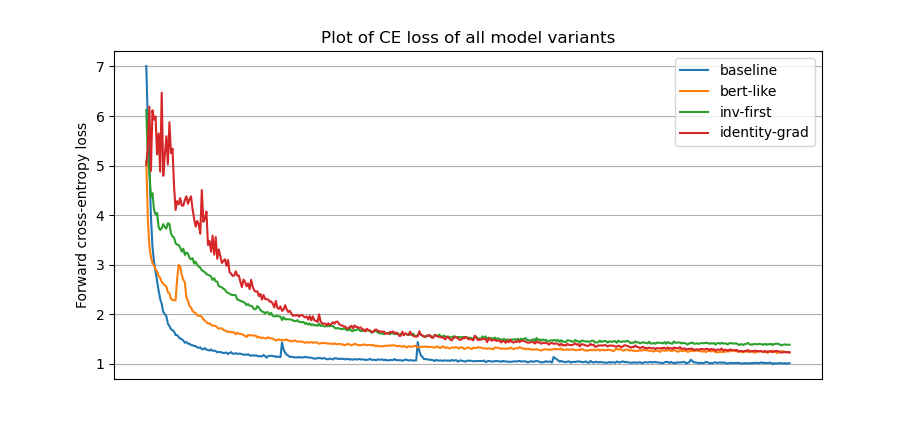
\includegraphics[width=\linewidth]{assets/inverse-lm/inverse_lm_variants_ce_loss.png}
    \caption{Cross-entropy loss value slowly improving during training}
    \label{fig:inverse_lm_variants_ce_loss}
\end{figure}


\subsection{First tokens distribution}
%% Dire che predire il primo token è too easy,
%% facendo vedere la distribuzione dei primi token (c'è il plot su Discord)
Looking at the results obtained when predicting the very first token with \texttt{inv-first}, we may ask if this result is really so good or there is something hiding behind those accuracies (\cref{table:tinystories__inversion_first_token_pad}).
Indeed, investigating the entropy that classifying the first token will have, we must see the distribution of the possible outcomes predicting that token in our particular dataset. This is visible in \cref{fig:tinystories_first_tokens_distribution}.
In the plot, tokens with less than 5,000 occurrences in the training dataset have been hidden for improved readability.
We can see that the first tokens are extremely imbalanced: summing up the occurrences of ``\emph{Once}'' and ``\emph{One}'' as the tokens in the very first position, we have covered almost every train sentence, which is pretty bad in our situation and will likely forge our results. Moreover, this motivates the top-2 accuracy for \texttt{inv-first} when predicting the first token, since having those two tokens as the most likely to be predicted, already makes the model performance result in a nearly-perfect accuracy.

In \cref{fig:tinystories_entropy_tokens_index} we can see that the most interesting and variable parts of text appear around the 20th token, where the entropy reaches values near 8.
Recall that the entropy in that plot is computed according to the formula of the Shannon entropy, where $i$ is the token index, $\mathcal{V}$ is the vocabulary and $p_i(x)$ is the probability of having the token $x$ at index $i$ of a randomly picked sentence in the training dataset:
\begin{equation}
\begin{split}
    H_i(x) &= - \sum_{x \in \mathcal{V}} p_i(x) \; log_2(p_i(x) + \varepsilon) \\
    \varepsilon &= 10^{-4} \; \text{For numerical stability of the } log
\end{split}
\label{eq:shannon_entropy}
\end{equation}

\begin{figure}[htbp]
    \centering
    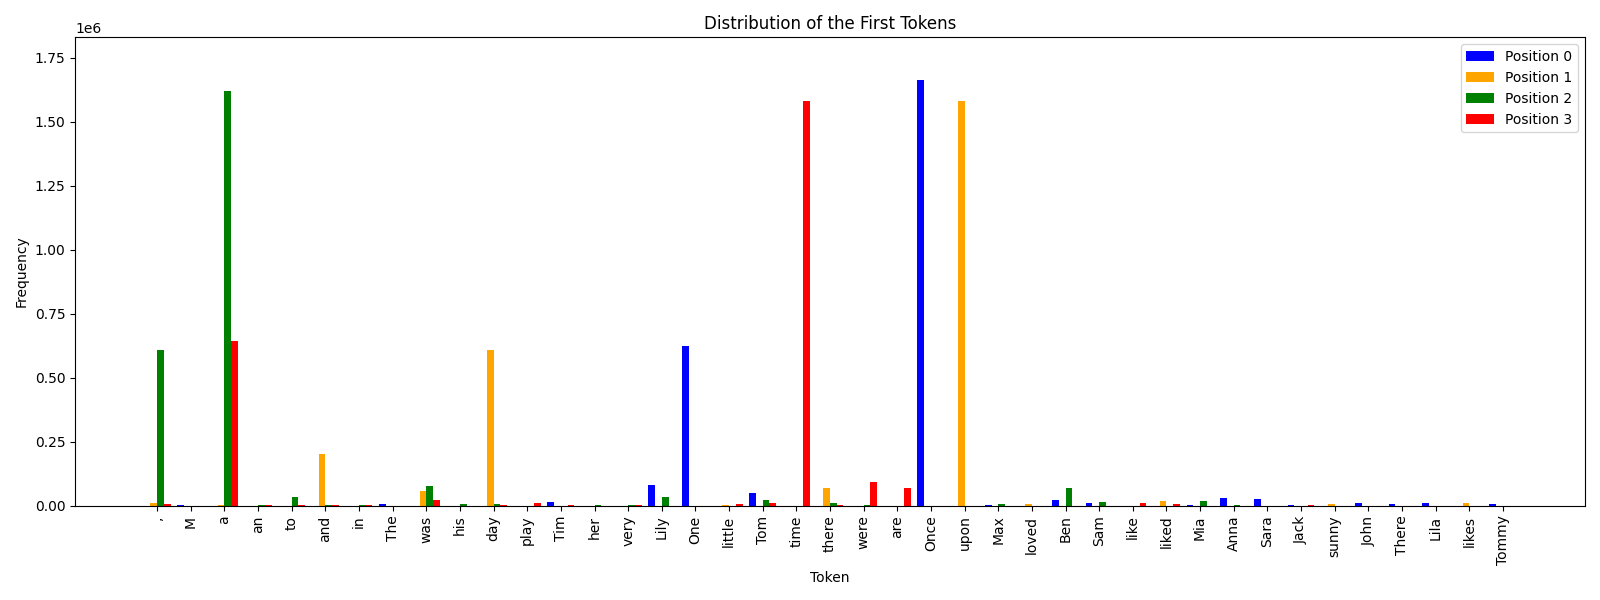
\includegraphics[width=\linewidth]{assets/inverse-lm/first_tokens_distribution.png}
    \caption{Distribution of tokens in the first positions of the sentences in the training set}
    \label{fig:tinystories_first_tokens_distribution}
\end{figure}

\begin{figure}[htbp]
    \centering
    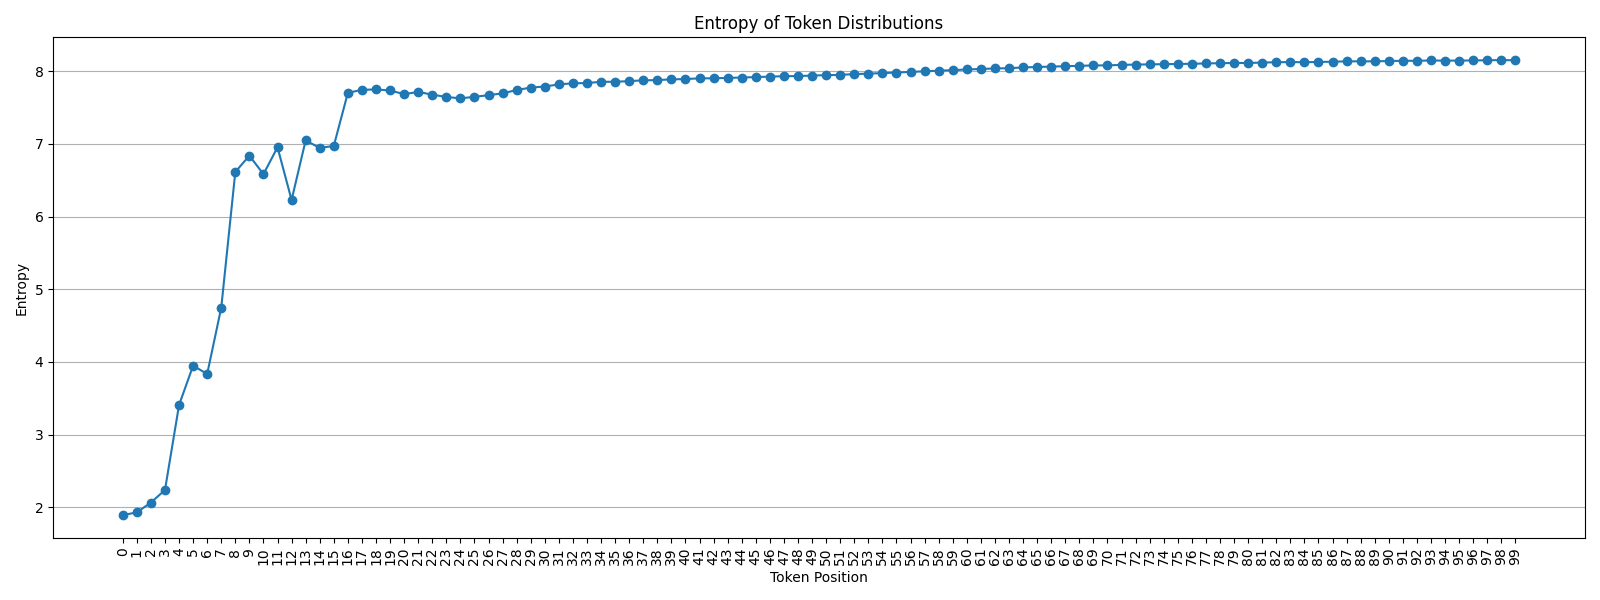
\includegraphics[width=\linewidth]{assets/inverse-lm/entropy_tokens_index.png}
    \caption{Entropy of tokens distribution at each index of the sentences in the training set}
    \label{fig:tinystories_entropy_tokens_index}
\end{figure}


\section{Inverting multiple tokens}
\label{sec:invert_sentence}
%% Dire che è stato fatto con top-k beam, descrivendo i test
As a direct consequence of the results in \cref{fig:tinystories_entropy_tokens_index},
it is mandatory to expand the evaluation on inverting multiple tokens autoregressively and going in middle positions in the text samples, instead of predicting the very first tokens as in the preliminary experiments.

% To do that, the procedure involved a \textbf{Beam Search}:
% \begin{enumerate}
%     \item Starting from a single sample $\bx$, let $k$ be the position to split the prefix and the suffix of the sample ($0 \leq k < n$), and $b$ the beam size: we used $k = 30$ and $b = 20$
%     \item Split the sample into the original prefix $\bx_p = \bx_{0:k}$ and the suffix $\bx_s = \bx_{k:n}$ given to the model
%     \item Let $\bX = \{ \bx \}$ be the set of sentences in the beam search
%     \item Compute the $b$ most probable tokens for the previous position, for each sample in $\bX$, according to the specific strategy and model used
%     \item Let $\bX =$ the $b$ generated samples with the lowest perplexity
%     \item Repeat the generation and filtering steps until a sufficiently long prefix has been generated
%     \item Return $\bx =$ the sample in $\bX$ with the lowest perplexity
% \end{enumerate}

The procedure follows a beam-search strategy, as detailed in \cref{alg:inversion_evaluation}, where candidate prefixes are iteratively expanded and filtered by perplexity until a coherent reconstruction emerges.

\begin{algorithm}[t]
\begin{algorithmic}[1]
\Require Input sample $\bx$ of length $n$, beam size $b$, split position $k$
\Ensure Inverted prefix $\bx_{\text{inv}}$
\State $\bx_p \gets \bx_{0:k}$, \quad $\bx_s \gets \bx_{k:n}$
\State Initialize beam set $\bX \gets \{\bx_s\}$
\While{inverted prefix not sufficiently long}
    \For{each sequence $\bx' \in \bX$}
        \State Compute the $b$ most probable previous tokens for the current position 
        \State Extend $\bx'$ with each candidate token
    \EndFor
    \State Update $\bX$ with the $b$ sequences having lowest perplexity
\EndWhile
\State \Return $\bx_{\text{inv}} \gets \arg\min_{\bx' \in \bX} \text{Perplexity}(\bx')$
\end{algorithmic}
\caption{Autoregressive Inversion Evaluation with Beam Search}
\label{alg:inversion_evaluation}
\end{algorithm}

\noindent
In the evaluation process, we considered only the combination of initialization strategy and model variant used in the specific training process. This means that the \texttt{Identity} has the unknown token initialized using the simple bigram, while other variants have it set to \texttt{<|pad|>}, since they reflect the same initialization strategy used during training. Of course, we cannot initialize the \texttt{Identity} model during inversion with the real token, as in training, because we do not know it yet. However, the best approximation we can do is to use a bigram model, which is pretty simple but also powerful to help the model invert better than starting from a totally random token or using a fixed \texttt{<|pad|>} because it has never observed it during training.

% \subsection{Qualitative results}
% \label{sec:invert_sentence__qualitative_results}
% The following results are qualitative, over a small set of examples, humanly picked among others to be discussed and take an interesting point. Of course, not all generated samples have these characteristics, but we aim to indicate that there is signal of something interesting happening, which may better evolve on bigger models or running the training process over a longer period of time.

% Testing the \texttt{bert-like} variant with the \texttt{pad} initialization strategy,
% there was one interesting sample, in \cref{tab:tinystories_bertlike_referring_future_context}.
% We can see that the last token of the predicted prefix is \emph{bug}, which is an animal as the original token \emph{frog}. In the same way, the predicted \emph{talking} is an adjective as the original \emph{friendly}. Finally, the bug is actually mentioned later in the story and it is mentioned that it talks, making \emph{sitting by talking bug} a plausible prefix. This is just something \textbf{sporadic}, that does not occur on a regular basis but rarely, which may be a signal that the model is somehow trying to go in that direction.

% \begin{table}[htbp]
% \centering
% \footnotesize
% \begin{tabular}{lp{0.85\linewidth}}
% \toprule
% $\bx$  & there was a hungry cat named Tom. Tom loved to listen to jazz music. \textbf{One sunny} \\
% $\bxa$ & happy sleepy lonely Bird off M W P friends walking free j o r tle d g \textbf{shining} \textbf{One upon sunny} \\
% \midrule
% $\by$  & day, Tom went outside to find some food. He \textbf{walked and walked} until he saw a big tree. In the tree, he saw a \textbf{bird} singing a jazz song. Tom climbed the tree to catch the bird. But the bird saw Tom and flew away. Tom was sad and regret that he tried to catch the bird. He just wanted to listen to the bird's jazz song. Then, something unexpected happened. The bird came back and said, [...] \\
% \tickrule
% $\bx$  & there was a lively boy named Tom. Tom loved to play with his toy rocket. \textbf{One day} \\
% $\bxa$ & P w la Tom played But happy W el k tle walking by One sit at The \textbf{To sunny day} \\
% \midrule
% $\by$  &  , he found a big rocket in his yard. He was so \textbf{happy}. \textbf{Tom} said to his mom, ``Look, Mom! A big rocket! \textbf{Can I play} with it?'' His mom smiled and said, ``Yes, Tom. But first, we need to polish it. It is very dirty.'' Tom and his mom cleaned the rocket. They used a soft cloth to polish it. The rocket shined like the \textbf{sun}. Tom played with the rocket all day long. He had so much fun. \\
% \bottomrule
% \end{tabular}
% \vspace{0.25cm}
% \caption{Some prefixes generated ($\bxa$) by penalized \texttt{bert-like} model can capture information from the suffix}
% \label{tab:tinystories_bertlike_referring_future_context}
% \end{table}

% Among the generated samples with this strategy, there are many prefixes that make no sense and often contain repeated tokens (\cref{tab:tinystories_bertlike_nonsense_low_ppl}). However, they have the peculiarity to have a \textbf{low perplexity}, even lower than the original and correct prefix. This indicates a strange behaviour in the model, where it outputs that the sentence composed by the predicted prefix and the given suffix is more probable than the string concatenation of the original prefix with the given suffix, where any human being would immediately say the opposite.

% \begin{table}[htbp]
% \centering
% \footnotesize
% \begin{tabular}{lp{0.85\linewidth}}
% \toprule
% $\bx$  & big, enthus \\
% $\bxa$ & doctor doctor doctor doctor doctor \\
% \midrule
% $\by$  & iastic smile. One day, Tim saw a sign near the park. The sign had a picture of a belt on it. [...] \\
% \tickrule
% $\bx$  & monkey decided to peek \\
% $\bxa$ & A w w P w \\
% \midrule
% $\by$  & around and see what it could find. The monkey was careful not to go too far and made sure to stay in a safe place. [...] \\
% \tickrule
% $\bx$  & trees. He had many \\
% $\bxa$ & La la jo la g \\
% \midrule
% $\by$  & friends in the forest, like the birds and the squirrels. They all liked to play together. [...] \\
% \bottomrule
% \end{tabular}
% \vspace{0.25cm}
% \caption{Nonsensical prefixes ($\bxa$) generated by \texttt{bert-like} model with low perplexity and lots of repeated tokens}
% \label{tab:tinystories_bertlike_nonsense_low_ppl}
% \end{table}

% \FloatBarrier

% Finally, the \texttt{identity} model variant looks promising, since with a \texttt{random} token initialization strategy (thus without using the bigram model) it is able to predict prefixes that do not show repeated, nonsensical, tokens repetitions. Above all, the prefix, separated from the sense of the suffix, often follows the grammatical pattern of a normal sentence, such as the order of adjectives, nouns, articles, verbs and so on (\cref{tab:tinystories_identity_random_init}).

% \begin{table}[H]
% \centering
% \footnotesize
% \begin{tabular}{lp{0.85\linewidth}}
% \toprule
% $\bx$  & smile. Anna liked to \\
% $\bxa$ & Lisa time ha peace there \\
% \midrule
% $\by$  & pretend that Lily was her sister, and they did everything together. One day, Anna's parent said, ``We have a surprise for you, Anna.'' [...] \\
% \tickrule
% $\bx$  & 's friend, Tim \\
% $\bxa$ & erry, who girl in \\
% \midrule
% $\by$  & , came over to play. Tim saw the toy heart and said, ``I want to play with the heart too!'' [...] \\
% \tickrule
% $\bx$  & trees. He had many \\
% $\bxa$ & heard that the tooth \\
% \midrule
% $\by$  & fairy would come and give her a coin for her tooth. She liked coins. She could buy candy with them. One night, Anna felt her tooth move a lot. [...] \\
% \bottomrule
% \end{tabular}
% \vspace{0.25cm}
% \caption{The predicted prefixes ($\bxa$, with \texttt{identity}) seem to follow a grammatical pattern}
% \label{tab:tinystories_identity_random_init}
% \end{table}


% \subsection{Penalizing repeated tokens}
% In most of the samples generated, even testing in different settings, we observed that the LLM tries to go in the direction of a nonsense prefix, repeating the same token predicted for first, without meaning or pattern, in order to favor of a lower perplexity.
% To prevent this degradation of the results, we tested changing the pruning criteria in the beam search. The new formula used to rank the generated samples is the following one and considers the perplexity of the overall sentence, concatenating the prefix with the suffix, and a \textbf{penalization factor} $D$ given by the number of repeated tokens.
% Ideally, this should let the beam search generate more diverse prefixes, instead of resulting in a sequence of repeated tokens.

% \begin{equation}
% \begin{split}
%     D(\bx_p) &= \text{length}(\bx_p) - \text{unique\_tokens}(\bx_p) \\
%     S(\bx_p, \bx_s) &= PPL(\bx_p || \bx_s) + \lambda D(\bx_p)
% \end{split}
% \end{equation}

% %%
% %% Discutere dei risultati con i file backward_dedup_*.txt
% %%
% The results shown an improvement in the \texttt{bert-like} model to capture some more details from the given suffix. In \cref{tab:tinystories_dedup_bertlike_future_context} it is possible to see that the generated prefix contains words like \emph{bird} that appears in the suffix, or \emph{shining} and \emph{sunny} reflecting the beautiful sunny day, mentioned multiple times in the rest of the story.
% In general, reading the generated prefixes we can see that they are in some strange way more or less \textbf{coherent} with the rest of the suffix text in some generated samples.

% % We cannot say the same analyzing the samples predicted with the  \texttt{inv-first} strategy (\cref{tab:tinystories_dedup_invfirst_nonsense}). They look like nonsense, but its fault may be associated with the training loop that \textbf{only looks at the very first token} in every sample, and according to what we previously observed, chances are that almost always it consists of 2 tokens ("\emph{Once}" and "\emph{One}").

% Last but not least, observing the generations provided by the \texttt{identity} model with a Bigram initialization, we observe that often a grammatical pattern is respected. However, on the contrary of what happens with the \texttt{bert-like} variant, the meaning between the generated suffix and the given suffix text do not seem to match or even leave a sparse sense of the meaning of the text the inversion was conditioned on.

% \begin{table}[htbp]
% \centering
% \footnotesize
% \begin{tabular}{lp{0.85\linewidth}}
% \toprule
% $\bx$  & smile. Anna liked to \\
% $\bxa$ &  there was a hungry cat named Tom. Tom loved to listen to jazz music. One sunny \\
% \midrule
% $\by$  & day, Tom went outside to find some food. He walked and walked until he saw a big tree. In the tree, he saw a bird singing a jazz song. Tom climbed the tree to catch the bird [...] \\
% \tickrule
% $\bx$  & there was a lively boy named Tom. Tom loved to play with his toy rocket. One day \\
% $\bxa$ & P w la Tom played But happy W el k tle walking by One sit at The To sunny day \\
% \midrule
% $\by$  & , he found a big rocket in his yard. He was so happy. Tom said to his mom, ``Look, Mom! A big rocket! Can I play with it?'' [...] \\
% \bottomrule
% \end{tabular}
% \vspace{0.25cm}
% \caption{Prefixes generated by penalized \texttt{bert-like} model capture information from the suffix}
% \label{tab:tinystories_dedup_bertlike_future_context}
% \end{table}

% % \begin{table}[htbp]
% % \centering
% % \footnotesize
% % \begin{tabular}{lp{0.85\linewidth}}
% % \toprule
% % $\bx$  & there was a little boy named Tom. He loved to play with his toys all day. One day \\
% % $\bxa$ & saw he liked They y har big upon She He Once small boy this park time there named One day \\
% % \midrule
% % $\by$  & Tom found a broken toy fire work in his room. It was red and blue, but it did not work anymore. Tom's friend, Sue, came to play. She saw the broken fire work and felt sad for Tom. [...] \\
% % \tickrule
% % $\bx$  & there was a little car named Timmy. Timmy lived in a small garage. He was a \\
% % $\bxa$ & The funny small boy this pa rk big little He liked In cat named there the time upon She Once was \\
% % \midrule
% % $\by$  & nervous car and always scared to leave the garage. Timmy had a big friend named Tom, who was a truck. Tom liked to help Timmy feel brave. One day, Tom said, "Timmy, let's go to the park and play with other cars." [...] \\
% % \bottomrule
% % \end{tabular}
% % \vspace{0.25cm}
% % \caption{Prefixes generated by penalized \texttt{identity} model, with bigram initialization, follow some grammatical pattern as well}
% % \label{fig:tinystories_dedup_identity_bigram}
% % \end{table}

% % \begin{table}[htbp]
% % \centering
% % \footnotesize
% % \begin{tabular}{lp{0.85\linewidth}}
% % \toprule
% % $\bx$  & Leopard went to the river to wash. He liked to be clean and shiny. The \\
% % $\bxa$ & Mum This W There Jimmy H D T N B Once Mark Hi M U J In A C An \\
% % \midrule
% % $\by$  & sun was up, and the sky was blue. The leopard was happy. As the leopard was hed in the river, a big fish jumped out of the water. The fish was very big and very fast. The leopard was surprised and a little scared [...] \\
% % \tickrule
% % $\bx$  & there was a farm with a big pumpkin patch. All the pumpkins were \\
% % $\bxa$ & There C T Tim Hi R U J N I M D Joe P He S O An L A \\
% % \midrule
% % $\by$  & big and round with bright orange skin. Everything was calm and quiet, until one day, when something strange happened - the pumpkins had all disappeared! [...] \\
% % \bottomrule
% % \end{tabular}
% % \vspace{0.25cm}
% % \caption{Prefixes generated by penalized \texttt{inv-first} model look like nonsense}
% % \label{tab:tinystories_dedup_invfirst_nonsense}
% % \end{table}

% \clearpage


\section{Gradients as directions}
\label{sec:ilm_inversion_gradients_token_directions}
%% Ciò che abbiamo fatto con identity-sum
In this section, we are going to propose a new model variant that follows the theoretical and more natural concept of gradients as directions.
Interestingly, we have already mentioned something of this kind in the introduction to this project: Perceptually Aligned Gradients (PAG, \citet{pag-imply-robustness}) can be interpreted as vectors that point in a direction chosen by the researcher, rather than being left free to go wherever they want.

Mathematically, gradients of the loss with respect to a component of the overall function, whether it be a weight parameter $\bw$, the input sample $\bx$, or any other intermediate value, indicate the delta to go to increase the loss.
Indeed, when training a simple neural network, the usual way is to use an optimizer to change the weights in the direction of the negative gradients of the loss function, multiplied by a learning rate and other advanced techniques, like momentum and so on.

The gradient on a token at some position $i$ is definitely interpretable, in a sequential model, 
as the direction to improve the current $i$-th token, to improve the overall loss function, given that its value has already ``seen'' the future elements to the sequence.

The main point of this reasoning is that it would be twisted to use the gradients as if they were the correct weights directly: no one would train a neural network as $\bw_{t+1} = \nabla_{\bw_t} \loss$, but the simplest and more general way to effectively train it is to change the weights as $\bw_{t+1} = \bw_t - \eta \nabla_{\bw_t} \loss$, thus exploiting gradients as directions.

The overall question that follows from this argument is: what could happen if we make the gradients concerning the input embedding be considered as a delta in the direction of the token itself?
To implement that, we take the already discussed model variants and apply a modification to its classification and training formulations.
Indeed, we classify on $\bx - \nabla_\bx \loss$, instead of directly on $\nabla_\bx \loss$ as we did in the previous sections of this chapter.
This allows the model to correctly use the gradients as directions towards what's a better value of the embedding token to lower the final loss. The full classification strategy is summarized in \cref{eq:sum_grads_ilm_classification}.

\begin{equation}
\begin{split}
    \loss_{CE} &= CE(\by_\text{true}, \by_\text{pred}) \\
    \bg_i &= \text{LayerNorm}(\bx_i - \nabla_{\bx_i}\loss_{CE}) \\
    \bz_i &= \bw_\text{LM\_head} \; \bg_i \\
    \mathbf{\hat{y}}_i &= \text{softmax}(\bz_i)
\end{split}
\label{eq:sum_grads_ilm_classification}
\end{equation}

\subbib{}
\end{document}